\documentclass[11pt]{article}
\usepackage[UTF8]{ctex}
\usepackage[a4paper]{geometry}
\geometry{left=2.0cm,right=2.0cm,top=2.5cm,bottom=2.5cm}

\usepackage{comment}
\usepackage{booktabs}
\usepackage{graphicx}
\usepackage{diagbox}
\usepackage{amsmath,amsfonts,graphicx,amssymb,bm,amsthm}
%\usepackage{algorithm,algorithmicx}
\usepackage[ruled]{algorithm2e}
\usepackage[noend]{algpseudocode}
\usepackage{fancyhdr}
\usepackage{tikz}
\usepackage{graphicx}
\usetikzlibrary{arrows,automata}
\usepackage{hyperref}
\hypersetup{
	colorlinks=true,
	linkcolor=blue,
	filecolor=blue,      
	urlcolor=blue,
	citecolor=cyan,
}			

\setlength{\headheight}{14pt}
\setlength{\parindent}{0 in}
\setlength{\parskip}{0.5 em}

\newtheorem{theorem}{Theorem}
\newtheorem{lemma}[theorem]{Lemma}
\newtheorem{proposition}[theorem]{Proposition}
\newtheorem{claim}[theorem]{Claim}
\newtheorem{corollary}[theorem]{Corollary}
\newtheorem{definition}[theorem]{Definition}
\newtheorem*{definition*}{Definition}

\newenvironment{problem}[2][Problem]{\begin{trivlist}
\item[\hskip \labelsep {\bfseries #1}\hskip \labelsep {\bfseries #2.}]}{\hfill$\blacktriangleleft$\end{trivlist}}
\newenvironment{answer}[1][Answer]{\begin{trivlist}
\item[\hskip \labelsep {\bfseries #1.}\hskip \labelsep]}{\hfill$\lhd$\end{trivlist}}

\newcommand\E{\mathbb{E}}
\newcommand\per{\mathrm{per}}


\title{Homework \#2}
\usetikzlibrary{positioning}

\begin{document}

\pagestyle{fancy}
\lhead{Peking University}
\chead{}
\rhead{Mathematical Foundations for the Information Age, 2025 Fall}

\begin{center}
    {\LARGE \bf Homework \#2}\\
    {Due: 2025-11-16 23:59 \quad$|$\quad 7 Problems, 100 Pts}\\
    {Name: Rainybunny, ID: 20120712}            % Write down your name and ID here.
\end{center}



\begin{problem}{1 (20')} Consider a cube $C$ with side length $1$ in $d$-dimensional space.
\begin{itemize}
    \item [(1)] (4') Write down the radius of a ball $B$ whose volume is equal to the cube's. You don't need to prove your result.
    \item [(2)] (16') When the centers of the cube $C$ and the ball $B$ are both at the origin, calculate the volume of their intersection when $d\to+\infty$.
    \item [] \textit{[Hint: Try to calculate $\mathbb{E}_{X\sim C}[\|X\|_2^2]$ and $Var_{X\sim C}[\|X\|_2^2]$. Then use Chebyshev's Inequality to analyze the concentration of $\|X\|_2^2$. You may use the Stirling's approximation}
    \begin{align*}
        \lim_{n\to+\infty}\frac{\Gamma(n+1)}{\sqrt{2\pi n}(n/\mathrm{e})^n}=1.\tag*{\textit{]}}
    \end{align*}
\end{itemize}
\end{problem}

\begin{answer} ~
\begin{itemize}
    \item [(1)] $r=\left(\frac{d\Gamma(d/2)}{2\pi^{d/2}}\right)^{\frac{1}{d}}$.
    \item [(2)] We use $\|\cdot\|$ as $\mathcal L2$-norm as default. Let distribution $U=\mathcal U[-\frac{1}{2},\frac{1}{2}]$, then
    $$
        \begin{aligned}
            \E_{X\sim C}(\|X\|^2) &= \E_{x_i\sim U[-\frac{1}{2},\frac{1}{2}]} \sum_{i=1}^d x_i^2\\
            &= \frac{d}{12}.
        \end{aligned}
    $$
    And
    $$
        \begin{aligned}
            \operatorname{Var}_{X\sim C}(\|X\|^2) &= \E(\|X\|^4)-\E(\|X\|^2)^2\\
            &= \E_{x_i\sim U}\left(\sum_{i=1}^{d} x_i^2\right)^2-\frac{d^2}{144}\\
            &= d(d-1)\E_{x,y\sim U} (x^2y^2)+d\E_{x\sim U}(x^4)-\frac{d^2}{144}\\
            &= \frac{d(d-1)}{144}+\frac{d}{80}-\frac{d^2}{144}\\
            &= \frac{d}{180}.
        \end{aligned}
    $$
    On the other hand, for $r_B^2$ when $d\to+\infty$, with \textit{Stirling's approximation}:
    $$
        \begin{aligned}
            r_B^{\frac{1}{d}} &= \frac{d\Gamma\left(\frac{d}{2}\right)}{2\pi^{\frac{d}{2}}}\\
            &\sim \frac{d\sqrt{2\pi\left(\frac{d}{2}-1\right)}\left(\frac{\frac{d}{2}-1}{\mathrm{e}}\right)^{\frac{d}{2}-1}}{2\pi^{\frac{d}{2}}}\\
            &= \frac{d\sqrt{2\pi\left(\frac{d}{2}-1\right)}}{2\pi}\cdot\left(\frac{\frac{d}{2}-1}{\pi\mathrm{e}}\right)^{\frac{d}{2}-1}\\
            &\to +\infty,
        \end{aligned}
    $$
    which implies
    $$
        r_B^2\to 1.
    $$
    Finally, with \textit{Chebyshev's Inequality},
    $$
        \Pr\left[ |\|X\|^2-\E(\|X\|^2)|\ge \frac{d}{4} \right] \le \frac{\frac{d}{180}}{\frac{d^2}{16}} = \frac{C}{d} \to 0,\quad C\in\mathbb R~\text{constant}.
    $$
    Therefore, for $X\sim C$, when $d\to+\infty$,
    $$
        V(B\cap C)=\Pr\left[\|X\|^2\le r_B^2\right]<\Pr\left[\|X\|^2<\frac{d}{12}\right]<\frac{C}{d}\to 0.
    $$
\end{itemize}
\end{answer}

\begin{problem}{2 (16')}
You select a PE class this term, so you need to complete a total of 85km of extracurricular exercise. There are only $n$ days before the deadline, but you still have $m$ kilometers remaining. To simplify your work, you can run at most 10km every day, but there is no lower bound. You are mindless when running, so the distance you run every day is uniformly random. In other words, the number of kilometers you run every day is a real number uniformly selected from range $[0,10]$. Prove that, the probability that you can complete $m$ kilometers in $n$ days, i.e., the probability that your total distance in $n$ days is greater than or equal to $m$ kilometers is 
\begin{align*}
    1-\sum_{i=0}^{\min(\lfloor m/10\rfloor,n)}\frac{(-1)^i}{i!(n-i)!}\left(\frac{m}{10}-i\right)^n.
\end{align*}
\end{problem}

\begin{answer} ~

    WLOG, let $m\gets m/10$ and I run at most 1km every day. Let the probability under our disccusion be $p(n,m)$, we need to prove
    $$
        p(n,m)=1-\sum_{i=0}^{\min(m,n)}\frac{(-1)^i}{i!(n-i)!}\left(m-i\right)^n.
    $$

    \textit{Easy to prove by induction. Anything more elegant?}

    Let $C_d=\{\boldsymbol{x}\in\mathbb R^d:0\le x_i\le 1\}$ be the unit cube, and $M_d(r)=\{\boldsymbol{x}\in\mathbb R^d:x_i\ge 0,~\sum_{i=1}^d x_i<r\}$ the non-negative part of Manhattan ($\mathcal L1$) sphere of radius $r$, in $d$-dimensional space. By definition,
    $$
        p(n,m)=\E_{X\sim C_n}[X\notin M_n(m)]=1-V(C_n\cap M_n(m)).
    $$

    In consideration of $V(C_n\cap M_n(m))$, applying \textit{Inclusion-Exclusion Principle} over restriction set $\{0\le x_i\le 1\}_{i=1}^n$ from $C_n$, we have
    $$
        V(C_n\cap M_n(m)) = \sum_{i=0}^{\min(m,n)}\binom{n}{i}(-1)^i V(M_n(m-i)),
    $$
    where $i$ enumerates the number of dimensions that disobey their restrictions. Recall (\underline{Homework \#1 Problem 8}) that $V(M_d(r)) = \frac{r^d}{d!}$. Therefore,
    $$
        p(n,m) = 1-\sum_{i=0}^{\min(m,n)}\binom{n}{i}(-1)^i \frac{(m-i)^n}{n!},
    $$
    which is what we want.
\end{answer}


\begin{problem}{3 (10')}
If $A$ is square, show that $AA^\top$ and $A^\top A$ are similar.

\textit{[Hint: Use the SVD of $A$.]}
\end{problem}

\begin{answer} ~

    Let $A=U\Sigma V^\intercal$, then
    $$
        AA^\intercal = (U\Sigma V^\intercal)(V\Sigma U^\intercal) = U\Sigma^2 U^\intercal,
    $$
    and
    $$
        A^\intercal A = (V\Sigma U^\intercal)(U\Sigma V^\intercal) = V\Sigma^2 V^\intercal.
    $$
    Let $C=VU^\intercal$ orthonormal, we find that
    $$
        C(AA^\intercal)C^\intercal = A^\intercal A\implies AA^\intercal \sim A^\intercal A.
    $$
\end{answer}

\begin{problem}{4 (12')}
Calculate the SVD of matrix $A$, where 
\begin{align*}
    A=\begin{pmatrix}
        -4&-6\\3&-8
    \end{pmatrix}.
\end{align*} 
You need to calculate it in two different ways.

\textit{[Hint: Use the definition of singular vectors, or consider $A^\top A$.]}
\end{problem}

\begin{answer} ~
\begin{itemize}
    \item[(a)] $A^\intercal A=\begin{pmatrix}25\\&100\end{pmatrix}$, $\lambda_1=100$, $v_1=\begin{pmatrix}0&1\end{pmatrix}^\intercal$, $\lambda_2=25$, $v_2=\begin{pmatrix}1&0\end{pmatrix}^\intercal$, $u_1=\frac{1}{\sigma_1}Av_1$, $u_2=\frac{1}{\sigma_2}Av_2$. Therefore,
    $$
        A = \begin{pmatrix}
            -\frac{3}{5} & -\frac{4}{5}\\
            -\frac{4}{5} & \frac{3}{5}
        \end{pmatrix} \begin{pmatrix}
            10 \\ & 5
        \end{pmatrix} \begin{pmatrix}
            & 1\\ 1
        \end{pmatrix}
    $$
    \item[(b)] Let $v=\begin{pmatrix}x & y\end{pmatrix}^\intercal$, then
    $$
        \|Av\|^2=(-4x-6y)^2+(3x-8y)^2=25x^2+100y^2.
    $$
    Obviously we can pick $v_1=\begin{pmatrix}0&1\end{pmatrix}^\intercal$, $\sigma_1=10$. Then $v_2=\begin{pmatrix}1&0\end{pmatrix}^\intercal\perp v_1$, $\sigma_2=5$. Finally we can calculate the result like (a).
\end{itemize}
\end{answer}

\begin{problem}{5 (16')}
Let $A=\sum_{i=1}^{r}\sigma_iu_iv_i^\top$ be the SVD of a rank-$r$ matrix $A$, let $A_k:=\sum_{i=1}^k\sigma_iu_iv_i^\top$ be the rank-$k$ approximation of $A$ for some $k<r$. 
\begin{itemize}
    \item [(1)] (4') Express the following quantities in terms of the singular values $\{\sigma_i,1\le i\le r\}$. You don't need to prove your result.
    \begin{itemize}
        \item [(a)] (2') $\|A_k\|_F^2$.
        \item [(b)] (2') $\|A_k\|_2^2$.
    \end{itemize}
    \item [(2)] (3') Prove that, $\sigma_k\le \frac{\|A\|_F}{\sqrt{k}}$ for $k=1,2,\cdots,r$.
    \item [(3)] (9') Suppose $A\in\mathbb{R}^{m\times m}$. Let $B=\sum_{i=1}^r\frac{1}{\sigma_i}v_iu_i^\top$.  
    \begin{itemize}
        \item [(a)] (6') Show that $BAx=x$ for all $x$ in the span of the right singular vectors of $A$. For this reason $B$ is sometimes called the pseudo inverse of $A$ and can play the role of $A^{-1}$ in many applications.
        \item [(b)] (3') Does $BAx=x$ always hold for all $x\in\mathbb{R}^m$? Prove or give a counterexample.
    \end{itemize}
\end{itemize}
\end{problem}

\begin{answer} ~
\begin{itemize}
    \item[(1)] $\|A_k\|_F^2=\sum_{i=1}^k\sigma_i^2$, $\|A_k\|_2^2=\sigma_1^2$.
    \item[(2)] It is a direct conclusion from $k\sigma_k^2 \le \sum_{i=1}^k \sigma_i^2 \le \sum_{i=1}^r\sigma_i^2 = \|A\|_F^2$.
    \item[(3-a)] For any $x\in\langle v_1,\cdots,v_r \rangle$, let $x=\sum_{i=1}^r a_iv_i$, and then
    $$
        \begin{aligned}
            BAx &= \sum_{i=1}^r\sum_{j=1}^r\sum_{k=1}^r \frac{1}{\sigma_i}v_iu_i^\intercal \cdot \sigma_j u_j v_j^\intercal \cdot a_k v_k\\
            &= \sum_{i=1}^r\sum_{j=1}^r\sum_{k=1}^r\frac{\sigma_j a_k}{\sigma_i}v_i(u_i^\intercal u_j)(v_j^\intercal v_k)\\
            &= \sum_{i=1}^r a_iv_i = x.
        \end{aligned}
    $$
    \item[(3-b)] No because $\operatorname{rank}BA\le\operatorname{rank}A=r$ and maybe $r<m$, where $\ker BA\neq\{0\}$. E.g.
    $$
        A=\begin{pmatrix}1\\&\end{pmatrix}=B,\quad x=\begin{pmatrix}\\1\end{pmatrix},\quad
        BAx=0\neq x.
    $$
\end{itemize}
\end{answer}

\begin{problem}{6 (16')}
In class, we introduced the best-fit subspace for a set of points. We extend this definition to probability densities instead of a set of points. If $P$ is a probability density in $\mathbb{R}^d$, then we define the best-fit $k$-dimensional subspace ($k\leq d$)
\begin{align*}
V_k=\arg\max_{V,\mathrm{dim}(V)=k}\E_{X\sim P}(|\mathrm{proj}(X,V)|^2),
\end{align*}
where $\mathrm{proj}(X,V)$ is the orthogonal projection of $X$ onto $V$.
\begin{itemize}
    \item [(1)] (6') Find out the best-fit $1$-dimensional subspace (i.e., a best-fit line through the origin) for probability density $\mathcal{N}\left(0,0,1,2,\frac{1}{2}\right)$.
    \item [] \textit{[Hint: Suppose random variable $(X_1,X_2)\sim\mathcal{N}\left(0,0,1,2,\frac{1}{2}\right)$, then we have}
    \begin{align*}
        X_1\sim\mathcal{N}(0,1),\;X_2\sim\mathcal{N}(0,2),\;\rho:=\frac{\mathbb{E}(X_1X_2)-\mathbb{E}(X_1)\mathbb{E}(X_2)}{\sqrt{Var(X_1)Var(X_2)}}=\frac12.\tag*{\textit{]}}
    \end{align*}
    \item [(2)] (10') Prove that, for $d$-dimensional Gaussian distribution $\mathcal{N}(\mu,I_d)$, a $k$-dimensional subspace is a best-fit subspace if and only if it contains $\mu$.
    \item [] \textit{[Hint: Suppose random variable $(X_1,\cdots,X_d)\sim\mathcal{N}(\mu,I_d)$, then we have $X_i\sim\mathcal{N}(\mu_i,1)$ and $X_1,\cdots,X_d$ are independent random variables.]}
\end{itemize}
\end{problem}

\begin{answer} ~
\begin{itemize}
    \item[(1)] \textit{Assume the parameter $2$ in $\mathcal N(0,2)$ refers to its $\sigma^2$ instead of $\sigma$.} Let the unit vector $u=\begin{pmatrix} \cos\theta & \sin\theta \end{pmatrix}^\intercal\in V$, $P=\mathcal N(0,0,1,2,\frac{1}{2})$. We have
    $$
        \begin{aligned}
            \E_{X\sim P}\|\text{proj}(X,V)\|^2 &= \E_{X\sim P}(X_1\cos\theta+X_2\sin\theta)^2\\
            &= \cos^2\theta\cdot \E_{X\sim P}(X_1^2)+\sin^2\theta\cdot\E_{X\sim P}(X_2^2)+2\cos\theta\sin\theta\cdot \E_{X\sim P}(X_1X_2)\\
            &= \cos^2\theta+2\sin^2\theta+\sqrt{2}\cos\theta\sin\theta\\
            &= \frac{3}{2}+\frac{\sqrt 3}{2}\left(-\frac{\sqrt 3}{3}\cos2\theta+\frac{\sqrt 6}{3}\sin2\theta\right).
        \end{aligned}
    $$
    Pick $u=\begin{pmatrix}\sqrt{\frac{3-\sqrt 3}{6}}&\sqrt{\frac{3+\sqrt 3}{6}}\end{pmatrix}^\intercal$ to maximize the expected norm of the projection.

    \item[(2)] Let $A=\begin{pmatrix}v_1&\cdots&v_k\end{pmatrix}$ formed by an orthonormal base of $V$, $P=\mathcal N(\mu,\boldsymbol{1}_d)$ and then
    $$
        \begin{aligned}
            \E_{X\sim P}\|A^\intercal X\|^2 &= \E_{X\sim P}\sum_{i=1}^k\left(\sum_{j=1}^d v_{ij}X_j\right)^2\\
            &= \sum_{i=1}^k\sum_{j=1}^d v_{ij}^2 (\E_{X\sim P}(X_j^2)-\E_{X\sim P}(X_j)^2) + \sum_{i=1}^k\sum_{p=1}^d\sum_{q=1}^dv_{ip}v_{iq}\E_{X\sim P}(X_p)\E_{X\sim P}(X_q)\\
            &= k+\|A^\intercal \mu\|^2.
        \end{aligned}
    $$
    So it is maximized iff $\|A^\intercal \mu\|^2\le\|\mu\|^2$ reaches equality, that is, $\mu\in V$.
\end{itemize}
\end{answer}

\begin{problem}{7 (10')}
Read in a photochrome and convert to a matrix. Perform a singular value decomposition of the matrix. Reconstruct the photo using only 1,2,4,16 singular values.
\begin{itemize}
    \item [(1)] Print the reconstructed photo. How good is the quality of the reconstructed photo? Write down your observations.
    \item [(2)] What percent of the Frobenius norm is captured in each case? Describe the way you calculate the captured Frobenius norm.
\end{itemize}

You need to include your original photochrome and all reconstructed photos in your answer and submit the code as an attachment.

\textit{[Hint: You may want to perform SVD on each channel.]}
\end{problem}

\begin{answer} ~
\begin{itemize}
    \item[(1)] See Figure \ref{fig:p7-recons}. The quality of reconstructed pictures increases with the number of singular dimensions used. To some degree, a $16$-channel reconstruction is capable to sketch a relatively large (1852$\times$2084) anime figure.
    \item[(2)] See Figure \ref{fig:p7-plot}. I calculated the Frobenius norm by definition (orange line) and by singular values (green line). They slightly mismatch because we have to clip tensor elements into $[0,255]$.
\end{itemize}

\begin{figure}[htbp]
\centering
\begin{minipage}{0.32\textwidth}\centering
    
\includegraphics[width=\linewidth]{p7-raw.png}\\
    \small (a) Original \footnote{Char.: 洛天依; Illus.: Ticoです.}
\end{minipage}\hfill
\begin{minipage}{0.32\textwidth}\centering
    
\includegraphics[width=\linewidth]{p7-approx-1.png}\\
    \small (b) 1 singular value
\end{minipage}\hfill
\begin{minipage}{0.32\textwidth}\centering
    
\includegraphics[width=\linewidth]{p7-approx-2.png}\\
    \small (c) 2 singular values
\end{minipage}

\vspace{0.8em}

\begin{minipage}{0.32\textwidth}\centering
    
\includegraphics[width=\linewidth]{p7-approx-4.png}\\
    \small (d) 4 singular values
\end{minipage}\hfill
\begin{minipage}{0.32\textwidth}\centering
    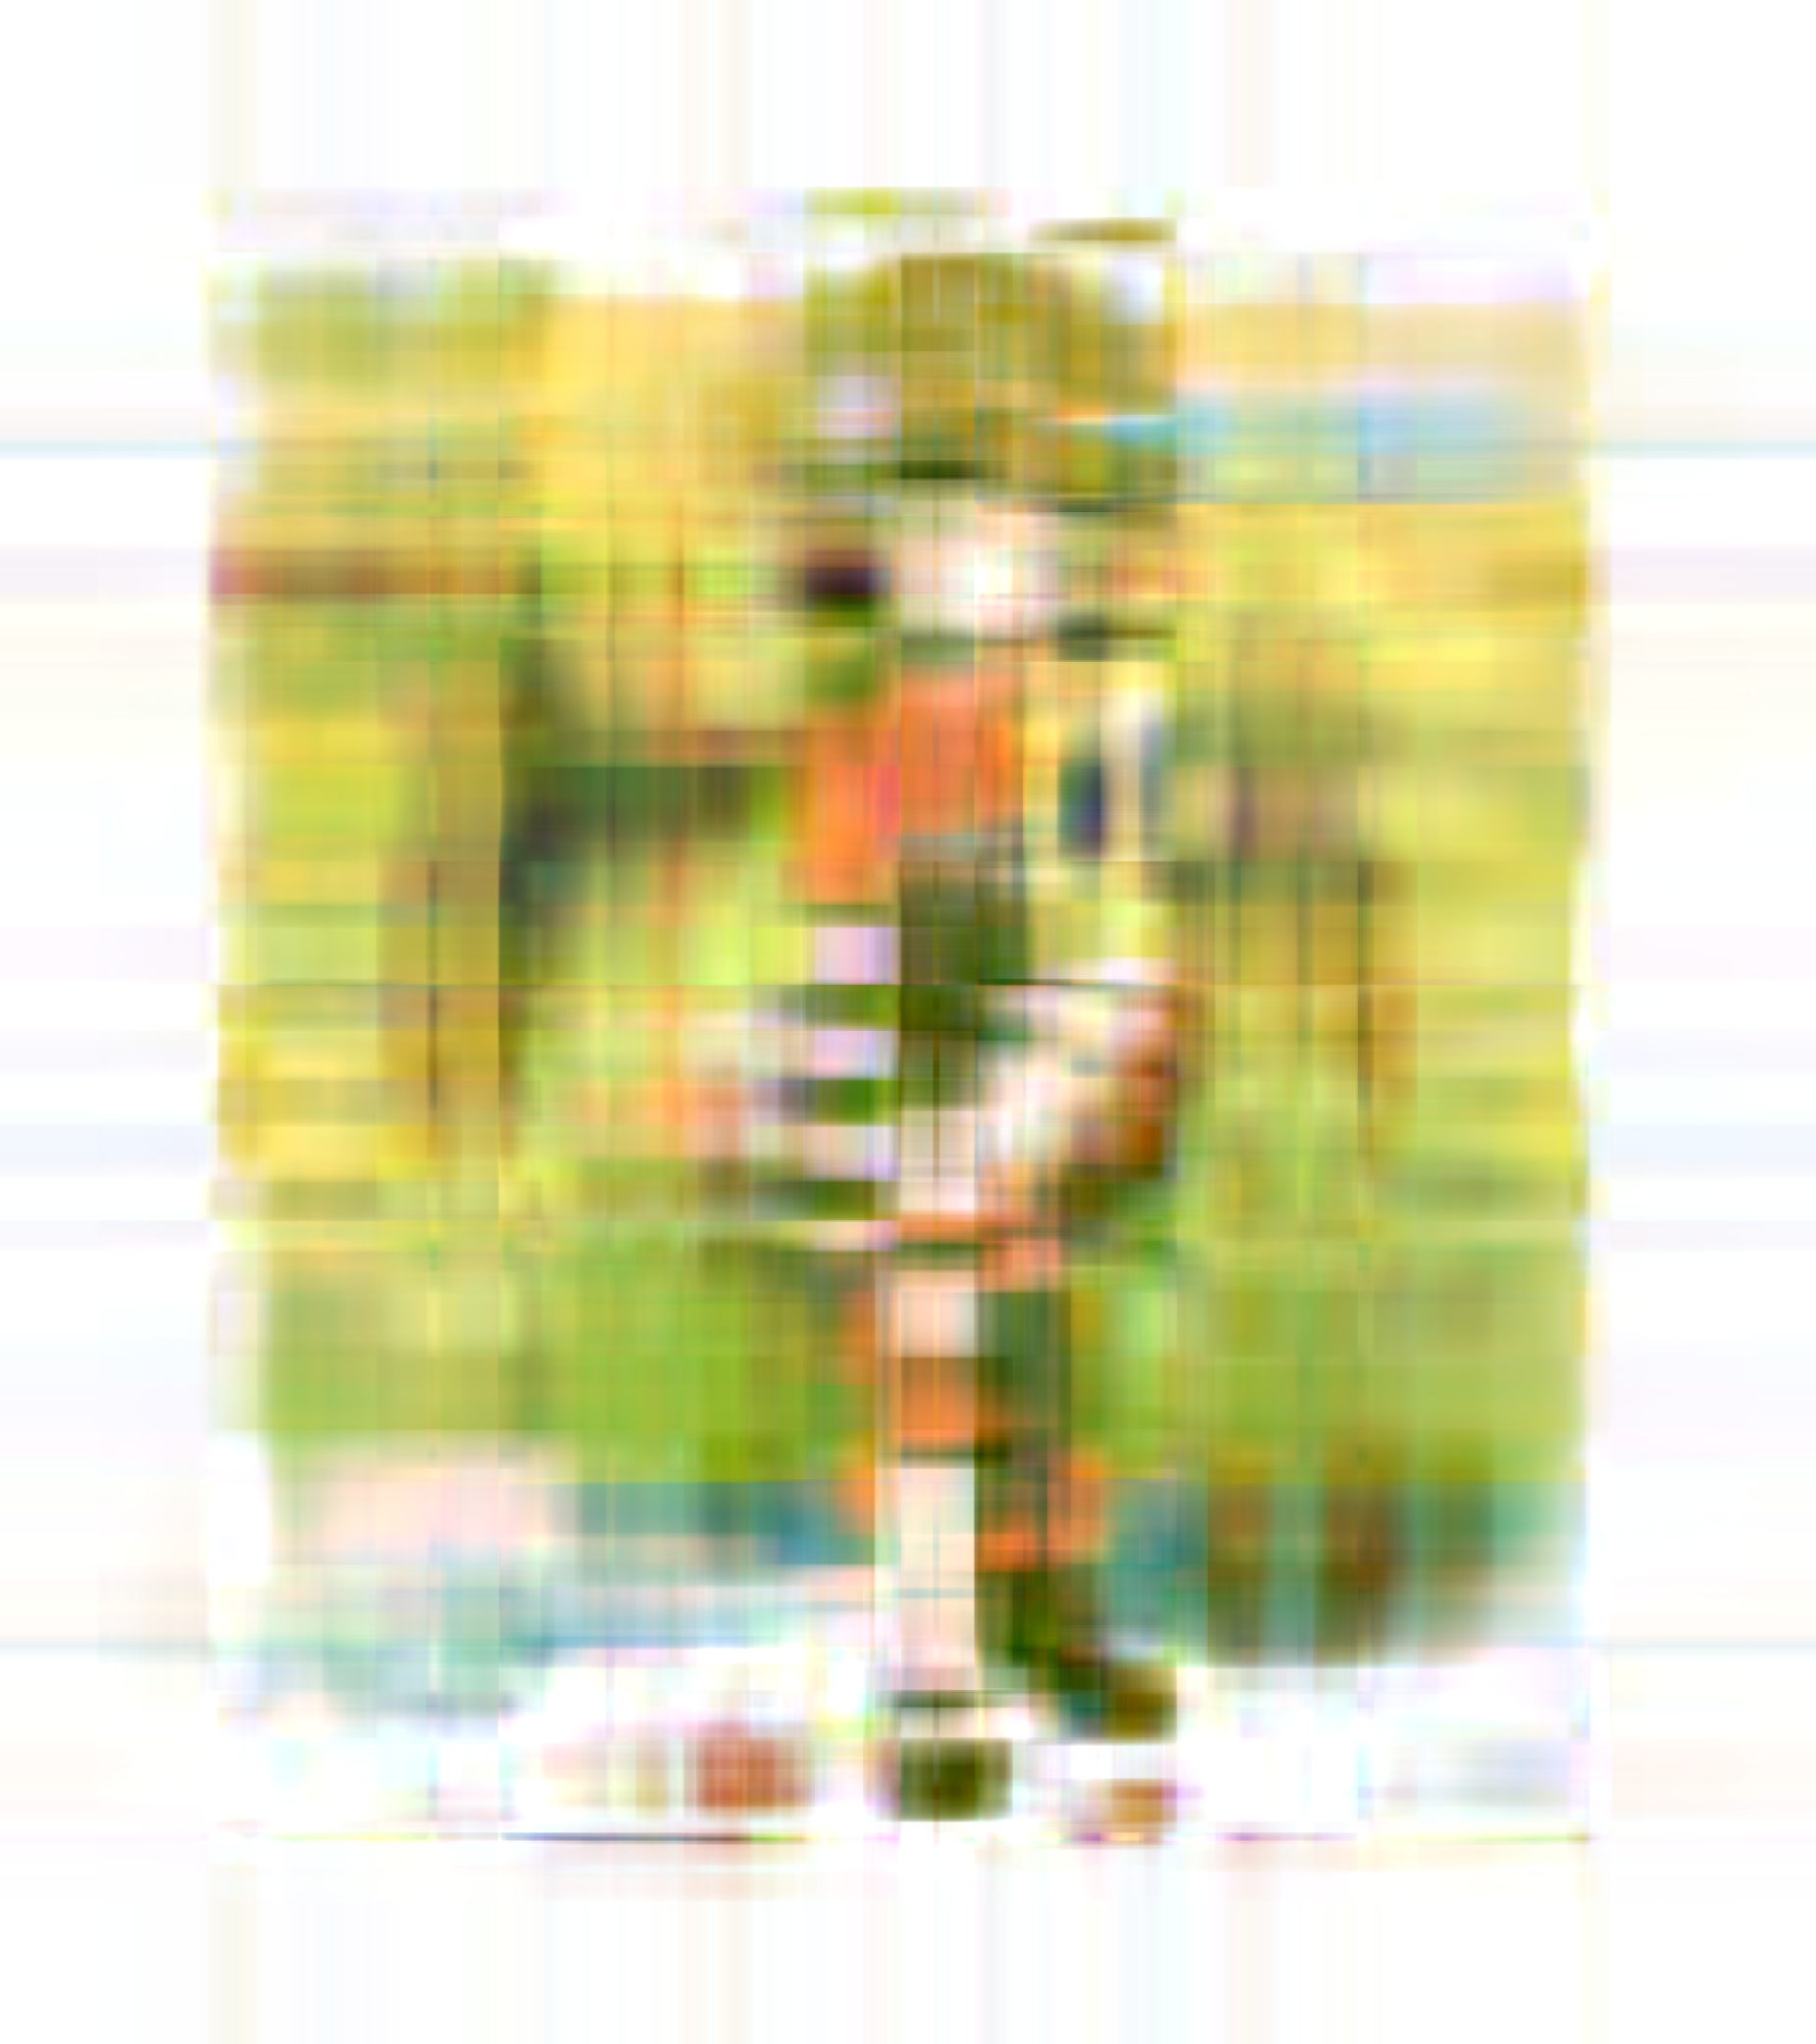
\includegraphics[width=\linewidth]{p7-approx-8.png}\\
    \small (e) 8 singular values
\end{minipage}\hfill
\begin{minipage}{0.32\textwidth}\centering
    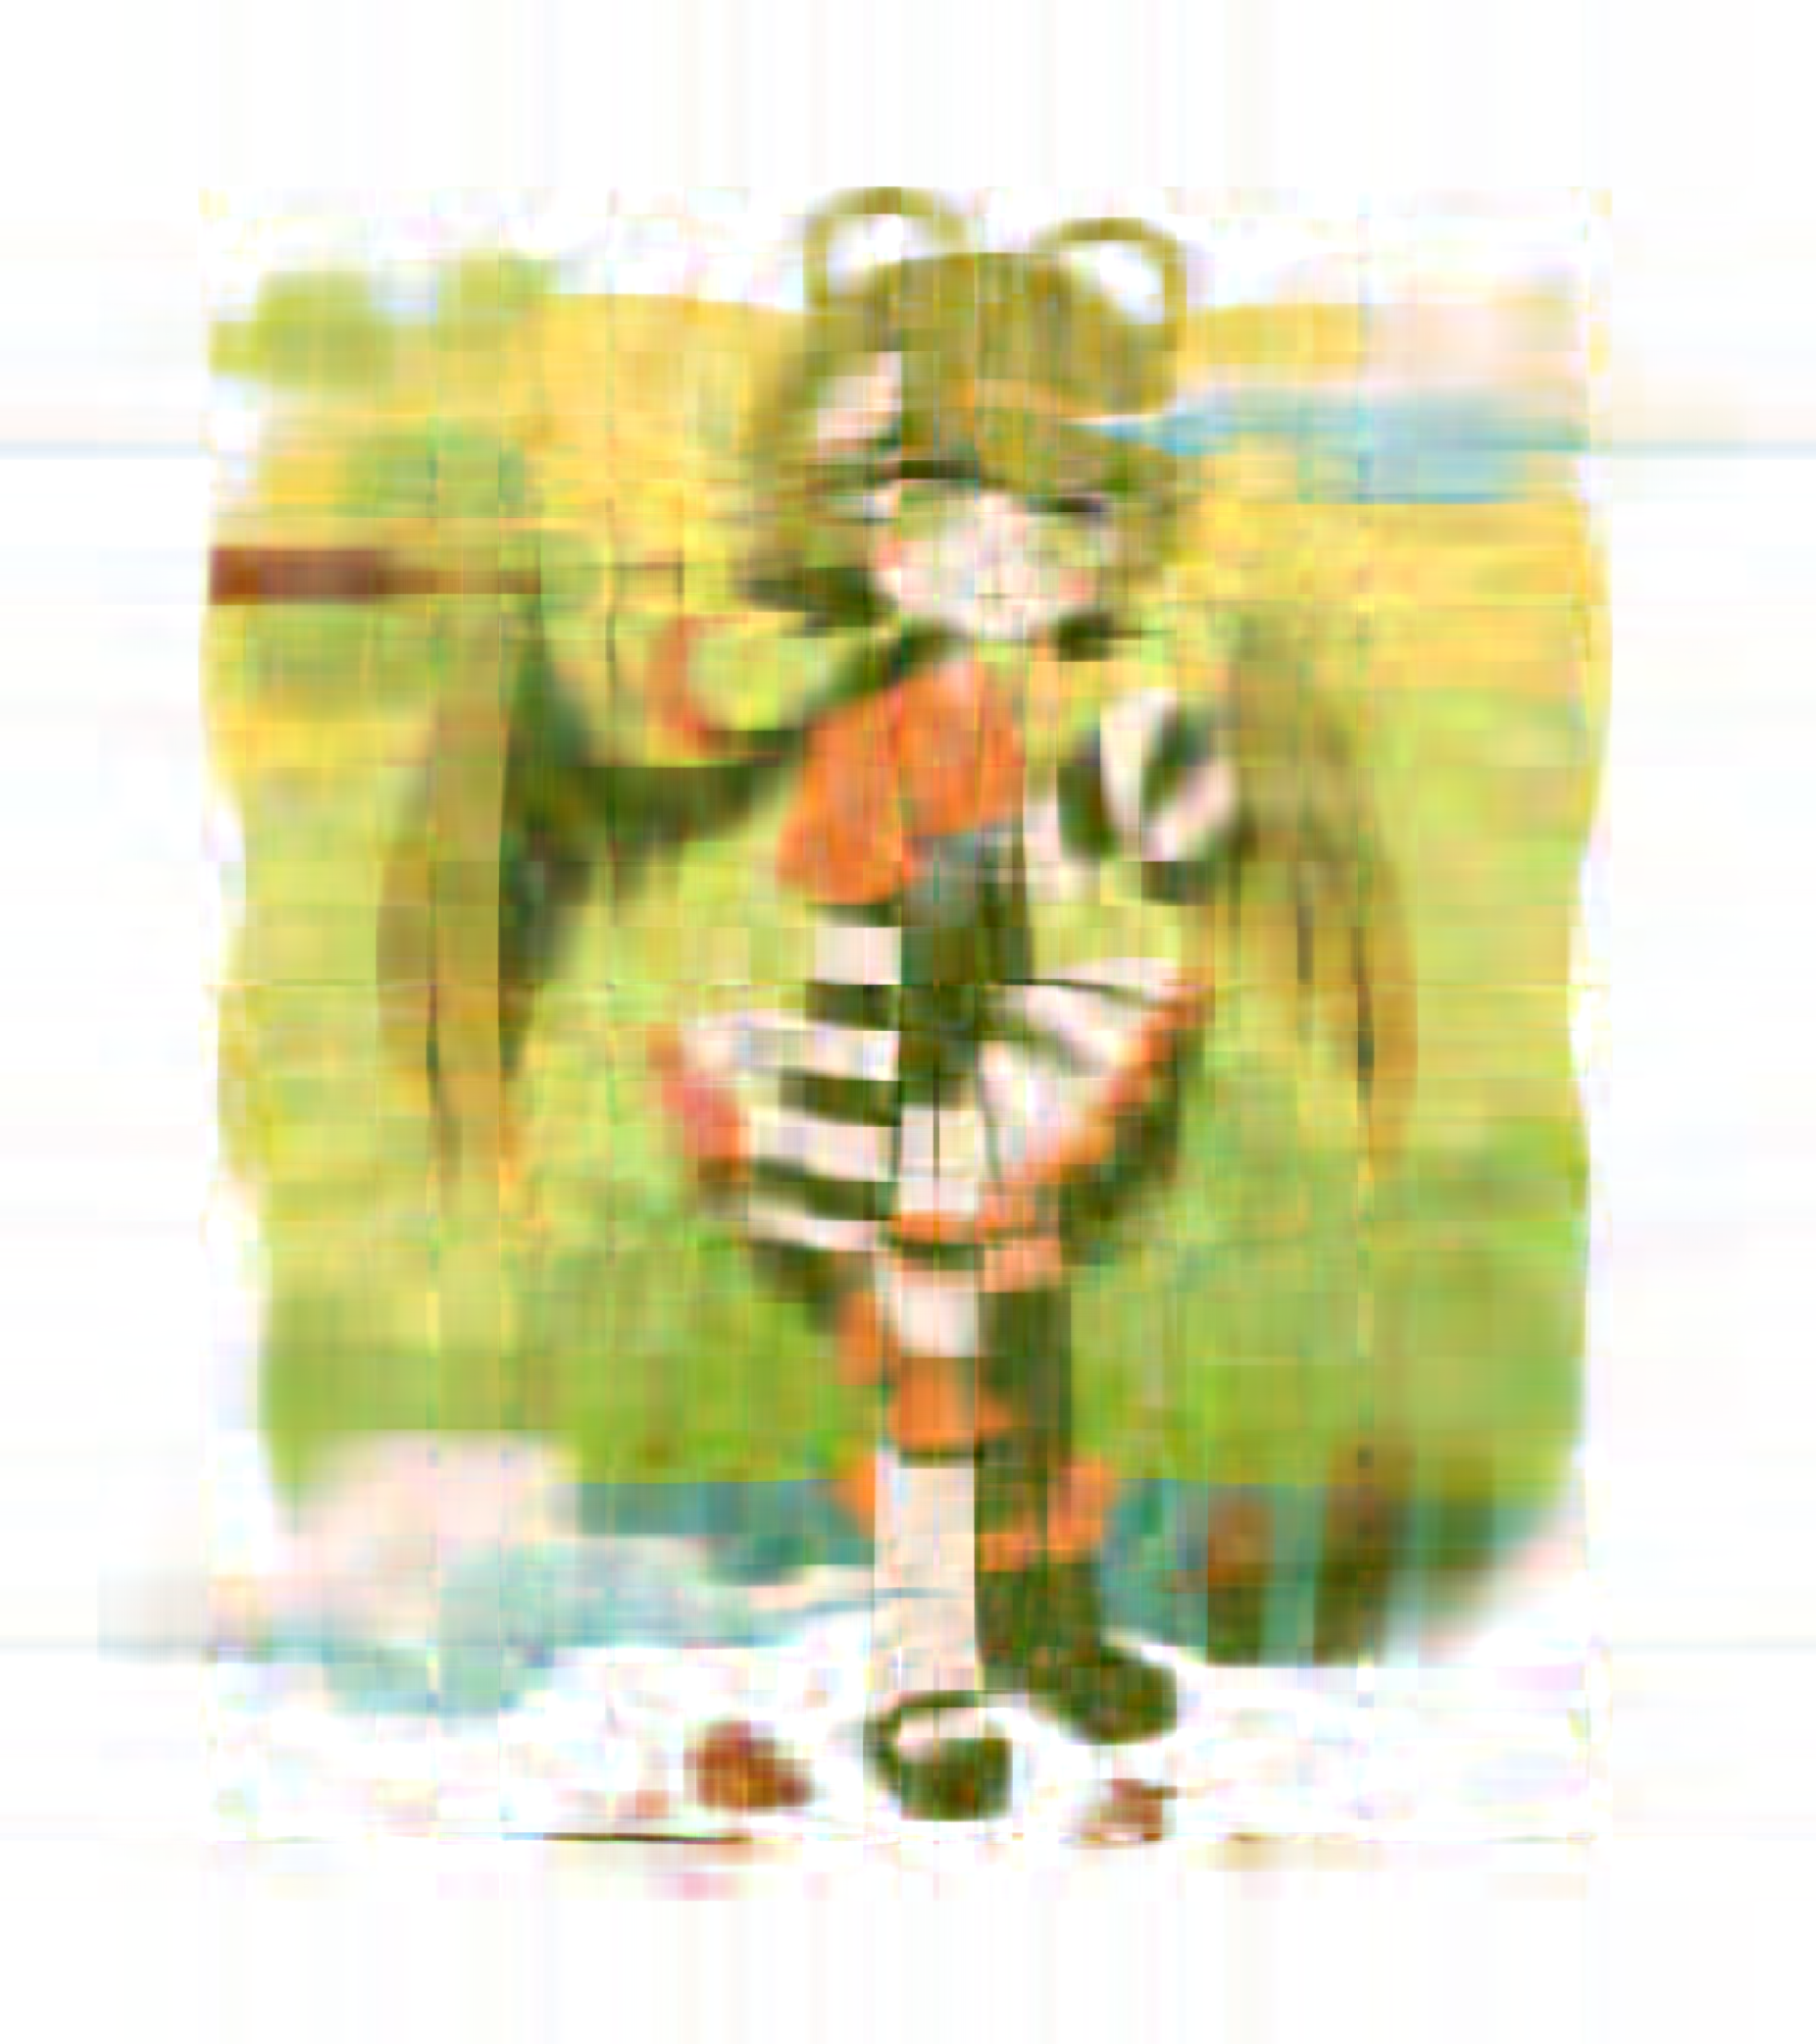
\includegraphics[width=\linewidth]{p7-approx-16.png}\\
    \small (f) 16 singular values
\end{minipage}

\caption{Reconstructed photos. Each image is scaled to fit the page; original resolution: 1852$\times$2084.}
\label{fig:p7-recons}
\end{figure}

\begin{figure}[htbp]
\centering
    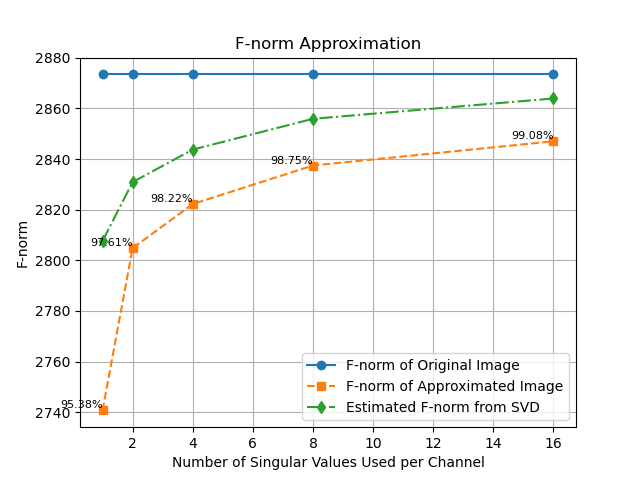
\includegraphics[width=0.6\textwidth]{p7-plot.png}\\
    \caption{Percent of Frobenius norm captured.}
    \label{fig:p7-plot}
\end{figure}

\end{answer}

\end{document}